\actTitle{4.2 - Trigonometric Functions Defined on the Unit Circle}

\videoLink{Section 4.2 day 1}{https://www.youtube.com/playlist?list=PLYHZK3b8UFw2_C72_BEthTH-k3sKuNAEb}
%\videoLink{Section 4.2 day 2}{https://www.youtube.com/playlist?list=PLYHZK3b8UFw1pcxMutFvlZct58eGZRjlC}

\noindent \textbf{Topics:}  unit circle, trigonometric functions, trigonometric identities, periodic\\

\noindent \textbf{Student Learning Outcomes:}
\begin{enumerate}
\item Students will be able to evaluate trigonometric functions using the unit circle.
\item Students will be able to determine domains of trigonometric functions.
\item Students will be able to use trigonometric identities.
\end{enumerate}

\hrule 

\bigskip

\subsection{Trigonometric Functions of Real Numbers} ~

\noindent
A \textbf{\underline{unit circle}} is a circle of radius 1 with center
at the origin.  The equation of a unit circle is:
$$x^2+y^2=1$$

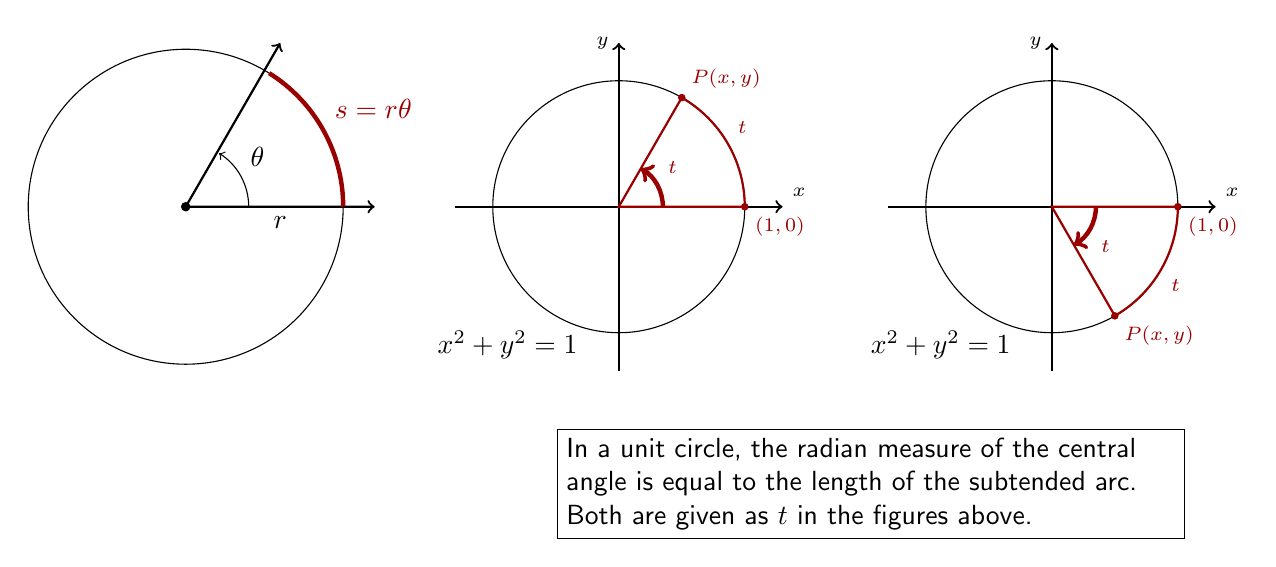
\begin{tikzpicture}[y=2cm, x=2cm,font=\sffamily]
     \begin{scope}[shift={(0,0)},scale=1]
          \draw[black] (0,0) circle(1);
          \draw[thick,<->] (1.2,0) -- (0,0)
               node[anchor=north,align=left,pos=0.5] {$r$}
              -- (60:1.2);
          \draw[thin,black,->] (0.4,0) arc (0:58:0.4)
              node[anchor=south west,pos=0.5] {$\theta$};
          \draw[ultra thick,red!60!black] (1,0) arc (0:58:1)
              node[anchor=south west,pos=0.5] {$s=r\theta$};
          \fill[black] (0,0) circle [radius=0.4ex];
     \end{scope}

     \begin{scope}[shift={(2.75,0)},scale=0.8]
       \draw[thick,->] (-1.3,0) -- (1.3,0) node[anchor=south west,font=\scriptsize] {$x$};
       \draw[thick,->] (0,-1.3) -- (0,1.3) node[anchor=east,font=\scriptsize] {$y$};
       \draw[black] (0,0) circle(1);
       \draw[thick,red!60!black] (60:1)
          -- (0,0) -- (1,0)
          node[anchor=north west,font=\scriptsize,align=left,pos=1.0] {$(1,0)$};
       \draw[thick,red!60!black] (1,0) arc (0:60:1)
          node[anchor=south west,font=\scriptsize,pos=0.5] {$t$};
       \draw[ultra thick,red!60!black,->] (.35,0) arc (0:60:.35)
              node[anchor=south west,font=\scriptsize,pos=0.5] {$t$};
       \fill[red!60!black] (1,0) circle [radius=0.4ex];
       \fill[red!60!black] (60:1) circle [radius=0.4ex]
                 node[anchor=south west,font=\scriptsize,align=left] {$P(x,y)$};
       \node[black,anchor=east] at (-0.25,-1.1) {$x^2+y^2=1$};
       \node[black,align=left,draw,text width=22em] at (2,-2.2)
          {In a unit circle, the radian measure of the central angle 
            is equal to the length of the subtended arc. Both are 
            given as $t$ in the figures above.};
     \end{scope}
   
     \begin{scope}[shift={(5.5,0)},scale=0.8]
       \draw[thick,->] (-1.3,0) -- (1.3,0) node[anchor=south west,font=\scriptsize] {$x$};
       \draw[thick,->] (0,-1.3) -- (0,1.3) node[anchor=east,font=\scriptsize] {$y$};
       \draw[black] (0,0) circle(1);
       \draw[thick,red!60!black] (-60:1)
          -- (0,0) -- (1,0)
          node[anchor=north west,font=\scriptsize,align=left,pos=1.0] {$(1,0)$};
       \draw[thick,red!60!black] (1,0) arc (0:-60:1)
          node[anchor=north west,font=\scriptsize,pos=0.5] {$t$};
       \draw[ultra thick,red!60!black,->] (.35,0) arc (0:-60:.35)
              node[anchor=north west,font=\scriptsize,pos=0.5] {$t$};
       \fill[red!60!black] (1,0) circle [radius=0.4ex];
       \fill[red!60!black] (-60:1) circle [radius=0.4ex]
                 node[anchor=north west,font=\scriptsize,align=left] {$P(x,y)$};
       \node[black,anchor=east] at (-0.25,-1.1) {$x^2+y^2=1$};
       \end{scope}

 \end{tikzpicture}

   \noindent\colorbox{blue!10}{%
   \parbox{\dimexpr\linewidth}%
   {%
     \textbf{Definitions of the trigonometric functions in terms of a
       unit circle.}

     If $t$ is a real number and $P(x,y)$ is a point on the unit
     circle corresponding to $t$, then
     \begin{eqnarray*}
       \begin{array}{rcl@{\hspace{4em}}rcl}
         \sin(t) & = & y, & \csc(t) & = & \frac{1}{y},~y\neq 0,\\ [10pt]
         \cos(t) & = & x, & \sec(t) & = & \frac{1}{x},~x\neq 0, \\ [10pt]
         \tan(t) & = & \frac{y}{x},~x\neq 0, & \cot(t) & = & \frac{x}{y},~y\neq 0.
       \end{array}
     \end{eqnarray*}
   }
 }


\newpage









\begin{enumerate}
\item Suppose that the real number $t$ corresponds to the point $P(-\frac{2}{3},-\frac{\sqrt{5}}{3})$ on the unit circle.  Evaluate the six trigonometric functions of $t$.
\begin{enumerate}
\item $\sin(t)=$\\[.5in]
\item $\cos(t)=$ \\[.5in]
\item $\tan(t)=$ \\[.5in]
\item $\csc(t)=$ \\[.5in]
\item $\sec(t)=$ \\[.5in]
\item $\cot(t)=$ \\[.5in]
\end{enumerate}

\subsection{Fundamental Trigonometric Identities} ~

\textbf{Reciprocal Identities:  }
$$\sin(\theta)=\frac{1}{\csc(\theta)} \quad \quad \cos(\theta)=\frac{1}{\sec(\theta)} \quad \quad \tan(\theta)=\frac{1}{\cot(\theta)}$$
Let's find three more:\\[.2in]

\textbf{Quotient Identities:  }
$$\tan(\theta)=\frac{\sin(\theta)}{\cos(\theta)} \quad \quad \cot(\theta)=\frac{\cos(\theta)}{\sin(\theta)}$$

\item Let $P(\frac{15}{17}, \frac{8}{17})$ be a point on the unit circle that correspond to $t$.  Find each of the six trig functions of $t$.\\[1.7in]

\item Use the $(x,y)$ coordinates in the unit circle to find the value of each trig function at the indicated real number $t$.\\

\begin{enumerate}
\item $\displaystyle \cos\Big(\frac{3\pi}{2}\Big)=$\\[.2in]
\item $\displaystyle \tan\Big(\frac{11\pi}{6}\Big)=$\\[.5in]
\item $\displaystyle \sec\Big(\frac{11\pi}{6}\Big)=$\\[.5in]
\item $\displaystyle \sin(-2\pi)=$\\[.2in]
\end{enumerate}

\item Evaluate the six trigonometric functions of the real number $t$.
\begin{enumerate}
\item $\displaystyle t=\frac{5\pi}{3}$
\newpage
\item $\displaystyle t=-\frac{5\pi}{4}$\vfill
\item $\displaystyle t=\pi$\vfill
\item $\displaystyle t=\frac{5\pi}{2}$\vfill
\end{enumerate}


\newpage

\subsection{Domains of the Trigonometric Functions} ~


\subsubsection{Pythagorean Identities} ~

$$\sin^2(t)+\cos^2(t)=1 \quad \quad \tan^2(t)+1=\sec^2(t) \quad \quad 1+\cot^2(t)=\csc^2(t)$$
\\

\item Given that $\tan(t)=\frac{12}{5}$ for $\pi < t < \frac{3\pi}{2}$, use an appropriate identity to find the value of $\sec(t)$.\\[2in]

\item Given that $\csc(t)=\frac{5}{4}$ for $\frac{\pi}{2} < t < \pi$, use an appropriate identity to find the value of $\cot(t)$.\\[2in]

\item Given a real number $t$, express $\sin(t)$ in terms of $\cos(t)$.\\[1.5in]

\newpage

\subsubsection{Even, Odd, and Periodic Properties} ~

   \noindent\colorbox{blue!10}{%
   \parbox{\dimexpr\linewidth}%
   {%
     \textbf{Even and odd trigonometric functions.}

     The cosine and secant functions are even:
     \begin{eqnarray*}
       \begin{array}{rcl@{\hspace{4em}}rcl}
         \cos(-t) & = & \cos(t), & \sec(-t) & = & \sec(t).
       \end{array}
     \end{eqnarray*}

     The sine, cosecant, tangent, and cotangent functions are odd:
     \begin{eqnarray*}
       \begin{array}{rcl@{\hspace{4em}}rcl}
         \sin(-t) & = & \sin(t), & \csc(-t) & = & \csc(t),\\ [10pt]
         \tan(-t) & = & \tan(t), & \cot(-t) & = & \cot(t).
       \end{array}
     \end{eqnarray*}

   }
 }


\item Use the unit circle to find the value of
  $\displaystyle \cos \Bigg(\frac{2\pi}{3}\Bigg)$ and odd trig
  functions to find the value of
  $\displaystyle \cos \Bigg(-\frac{2\pi}{3}\Bigg)$.

\vfill
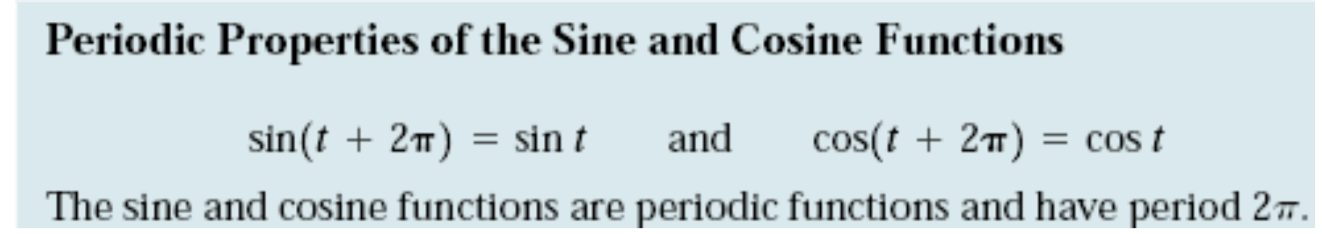
\includegraphics[scale=.6]{periodic1}\\
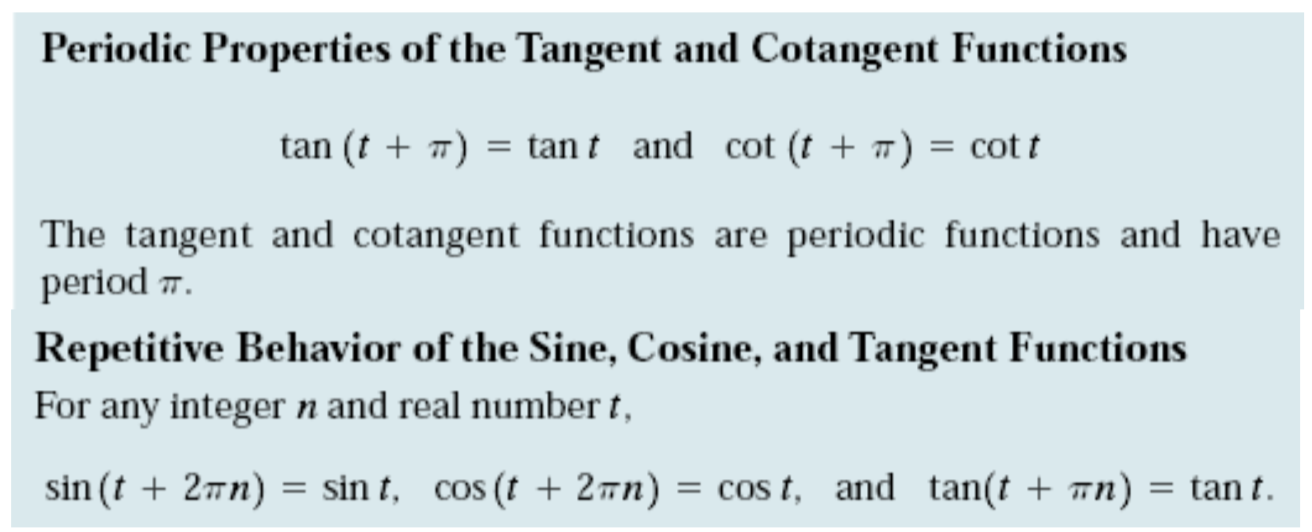
\includegraphics[scale=.6]{periodic}\\

\newpage
\item Given $\displaystyle \sin\Bigg(\frac{\pi}{12}\Bigg)=\frac{\sqrt{6}-\sqrt{2}}{4}$, determine the value of $\displaystyle \sin \Bigg( \frac{49\pi}{12} \Bigg)$.

\vfill
\item Use properties of trigonometric functions to simplify $\tan(-3t)-\tan(-3t+\pi)$.
\vfill

\subsubsection{Approximate Trigonometric Functions on a Calculator} ~

\item Use a calculator to approximate the function values.  Round to 4 decimal places.
\begin{enumerate}
\item $\displaystyle \cos \Bigg( \frac{2\pi}{7} \Bigg)$\\
\item $\csc(0.92)$\\[.2in]
\end{enumerate}



\end{enumerate}

\noindent \textbf{Student Learning Outcomes Check}

\begin{enumerate}
\item Can you evaluate trigonometric functions using the unit circle?
\item Can you determine domains of trigonometric functions?
\item Are you able to use trigonometric identities?

\end{enumerate}

\noindent \textbf{If any of your answers were no, please ask about these topics in class.}


